\documentclass{article}
\usepackage{graphicx} % Required for inserting images
\usepackage{amsmath}
\usepackage{xcolor}
\usepackage{float}
\usepackage{listings}
\usepackage{xcolor}

\lstset{
    % change caption to be below the listing
    % choose appropriate font style.
    captionpos=b,
  basicstyle=\footnotesize\ttfamily,
  numbers=left,
  numberstyle=\tiny,
  stepnumber=1,
  numbersep=8pt,
  frame=single,
  breaklines=true,
  tabsize=2,
  showstringspaces=false,
  keywordstyle=\color{blue},
  commentstyle=\color{gray},
  stringstyle=\color{teal},
}

\title{1D Diffusion self similar solution}
\author{Yuval.Kochavi And Tal Ramot}
\date{November 2025}

\begin{document}

\maketitle

\section{Adding global multiplier $\chi$ }
Notice that when $\chi\to \infty$, the problem will return "black" - i.e. there is a strong correlation between the radiation and the matter, and the system achieves equilibrium as $U\approx E$ . It also means that the matter is a perfect absorber and emitter. 
The equations for $E(x,\tau),\;U(x,\tau)$ with a global multiplier are

\begin{equation}
\frac{\partial E(x,\tau)}{\partial \tau} =\frac{\partial^2E(x,\tau)}{\partial x^2} + \chi(U(x,\tau) - E(z,\tau)),
\end{equation}

\begin{equation}
\frac{\partial U(x,\tau)}{\partial \tau} =\chi( E(x,\tau) - U(x,\tau))
\end{equation}
Using implicit finite differencing, one gets:

\begin{equation}
\frac{E_i^{n+1} - E_i^n}{\Delta \tau} = \frac{E_{i+1}^{n+1} - 2E_i^{n+1} + E_{i-1}^{n+1}}{(\Delta x)^2} + \chi(U_i^{n+1} - E_i^{n+1}),
\end{equation}
\begin{equation}
\frac{U_i^{n+1} - U_i^n}{\Delta \tau} = \chi(E_i^{n+1} - U_i^{n+1}),
\end{equation}
The second equation is local - solve for $U_i^{n+1}$:
\begin{equation}
    (1+\chi\Delta \tau) U_i^{n+1} - \chi \Delta \tau E_i^{n+1} = U_i^n
\end{equation}
\begin{equation}
    U_i^{n+1} = \frac{\chi\Delta \tau E_i^{n+1} + U_i^n}{1+\chi\Delta \tau}
\end{equation}
Now define $\alpha = \frac{\chi\Delta \tau}{1+\chi\Delta \tau}$, $\lambda = \frac{\Delta \tau}{(\Delta x)^2}$ and substitute into the first equation, reaching \underline{the exact same} equation as for the case $\chi=1$
explained in $\texttt{1D Diffusion Linear.tex}$ file.
\begin{equation}
(1+2\lambda+\alpha) E_i^{n+1} - \lambda E_{i+1}^{n+1} - \lambda E_{i-1}^{n+1} = E_i^n + \alpha U_i^n
\end{equation}
and from here on, the solution is exactly the same as in the previous file.
\section{Self-Similar Equation}
Now we are going to $\boldsymbol{neglect}$ the assumption $C_V\sim T^3$ that makes the equation linear. Define $T=T_m$ and $\boxed{U_R(T) = aT^4}$. We also denote $\beta = \frac{\partial U_r}{\partial U_m}$ the equations now take the form:
\begin{equation}
    \frac{\partial{E}}{\partial t}+\frac{\partial F}{\partial  z} = \chi c\sigma(U_R-E) 
\end{equation}
\begin{equation}
    \frac{\partial U_m}{\partial t}=-\chi c\sigma (U_R-E)\Rightarrow
    \frac{1}{\beta} \frac{\partial U_R}{\partial t}=-\chi c\sigma (U_R-E)
\end{equation}
\begin{equation}
    F=-D\frac{\partial E}{\partial z}\;\;\;\;\left(D=\frac{c}{3\sigma(T)}\right)
\end{equation}
The unknowns here are $E(z,t),U_R(z,t)$ and the coefficients $D(T),\beta(T)$ depend on the temperature, which is a function of $U_R$.
In addition, $U_m$ is also a function of $T$ so it is also solvable from $U_R$ (and we will use that in the simulation).

\section{Self-similar relations and unit analysis}
\subsection{Basic relations}
We assume the following self-similar relations for the opacity and the heat capacity.
Equations (2a),(2b) in the Shussman-Heizler paper:
\begin{equation}
    \frac{1}{\kappa_R} = g T^\alpha \rho^{-\lambda}
\end{equation}
\begin{equation}
    e = f T^\gamma \rho^{-\mu}
\end{equation}
% alarm bells icon at the beginning of the line
where $e$ is the specific internal energy, which means the material energy density is:
\begin{equation}
    U_m(T) = \rho e = f T^\gamma \rho^{-\mu + 1}
\end{equation}
\subsection{Relations for D(T), $\beta$(T)}
Using the definitions of $D,\beta$ and the self-similar relations for $\kappa_R,e$, we can find the relations for $D(T),\beta(T)$.
\begin{gather}
    D(T)=\frac{c}{3\sigma}=\frac{c}{3}gT^\alpha\rho^{-\lambda -1} \\
    \beta(T) = \frac{\partial U_R}{\partial U_m} = \frac{4aT^3}{f\gamma T^{\gamma-1}\rho^{-\mu+1}}=\frac{4a\rho^{\mu-1}}{f\gamma }T^{4-\gamma}
\end{gather}
from $U_m(T)$, $D(T)$ and $\beta(T)$, the simulation would be able to calculate the coefficients at each time step (see subsection 4.1).

\subsection{Unit analysis and Given Constants Values}
% Table 1: Initial and Boundary Conditions
\subsection{Initial and Boundary Conditions}
\renewcommand{\arraystretch}{1.5}
\begin{center}
\begin{tabular}{|l|c|c|}
    \hline
    \textbf{Parameter} & \textbf{Symbol} & \textbf{Value} \\
    \hline
    Initial material temperature (Kelvin) & $T_{\mathrm{material,0}}^{\mathrm{K}}$ & 300 K \\
    \hline
    Boundary bath temperature (Kelvin) & $T_{\mathrm{bath}}^{\mathrm{K}}$ & $10^6$ K \\
    \hline
    Initial material temperature (HeV) & $T_{\mathrm{material,0}}$ & $2.59 \times 10^{-4}$ HeV \\
    \hline
    Boundary bath temperature (HeV) & $T_{\mathrm{bath}}$ & 0.862 HeV \\
    \hline
    Speed of light & $c$ & 30 cm/ns \\
    \hline
    Global multiplier & $\chi$ & $10^5$ \\
    \hline
\end{tabular}
\end{center}
\renewcommand{\arraystretch}{1}

% Table 2: Simulation Grid and Time Parameters
\subsection{Simulation Grid and Time Parameters}
\renewcommand{\arraystretch}{1.5}
\begin{center}
\begin{tabular}{|l|c|c|}
    \hline
    \textbf{Parameter} & \textbf{Symbol} & \textbf{Value} \\
    \hline
    Domain length & $L$ & $10^{-4}$ cm \\
    \hline
    Number of spatial grid points & $N_z$ & 1000 \\
    \hline
    Spatial step size & $\Delta z$ & $10^{-7}$ cm \\
    \hline
    Final simulation time & $t_{\mathrm{final}}$ & 5.0 ns \\
    \hline
    Time step & $\Delta t$ & $5.0 \times 10^{-4}$ ns \\
    \hline
    Number of time steps & $N_t$ & 10001 \\
    \hline
\end{tabular}
\end{center}
\renewcommand{\arraystretch}{1}

% Table 3: Physical Constants and Unit Conversions
\subsection{Physical Constants and Unit Conversions}
\renewcommand{\arraystretch}{1.5}
\begin{center}
\begin{tabular}{|l|c|c|}
    \hline
    \textbf{Constant} & \textbf{Symbol} & \textbf{Value} \\
    \hline
    Electron volt to Joule & eV [SI] & $1.60218 \times 10^{-19}$ J \\
    \hline
    Erg per Joule & $erg/J$ & $10^7$ erg/J \\
    \hline
    Electron volt (erg units) & eV [cgs] & $1.60218 \times 10^{-12}$ erg \\
    \hline
    Hundred electron volt & HeV [cgs] & $1.60218 \times 10^{-10}$ erg \\
    \hline
    Boltzmann constant (Joule) & $k_B$ [SI] & $1.38065 \times 10^{-23}$ J/K \\
    \hline
    Boltzmann constant (erg) & $k_B$ [cgs] & $1.3805 \times 10^{-16}$ erg/K \\
    \hline
    Kelvin per HeV & $K/\mathrm{HeV}$ & $1.1605 \times 10^6$ K/HeV \\
    \hline
    Radiation constant (Kelvin) & $a [SI]$ & $7.5646 \times 10^{-15}$ erg/(cm$^3$K$^4$) \\
    \hline
    Radiation constant (HeV) & $a [cgs]$ & $1.377 \times 10^{11}$ erg/(cm$^3$HeV$^4$) \\
    \hline
\end{tabular}
\end{center}
\renewcommand{\arraystretch}{1}

% Table 4: Gold EOS Self-Similar Parameters
\subsection{Gold EOS Self-Similar Parameters}
\renewcommand{\arraystretch}{1.5}
\begin{center}
\begin{tabular}{|l|c|c|l|}
    \hline
    \textbf{Parameter} & \textbf{Symbol} & \textbf{Value} & \textbf{Description} \\
    \hline
    Specific energy coefficient & $f$ & $3.4 \times 10^{13}$ & [erg/g] \\
    \hline
    Opacity coefficient & $g$ & $1.389 \times 10^{-4}$ & $1/7200$ \\
    \hline
    Opacity exponent & $\alpha$ & 1.5 & -- \\
    \hline
    Specific energy exponent & $\gamma$ & 1.6 & -- \\
    \hline
    Opacity density exponent & $\lambda$ & 0.2 & -- \\
    \hline
    Specific energy density exponent & $\mu$ & 0.14 & -- \\
    \hline
    Material density & $\rho$ & 19.32 & g/cm$^3$ \\
    \hline
\end{tabular}
\end{center}
\renewcommand{\arraystretch}{1}




\section{Preparations For the Finite Difference Scheme}
\subsection{Boundary and Initial Conditions}
\underline{Initial Conditions}: The inital temperature is $T_m = T = T_{material-0}$ everywhere, which means:
\begin{equation}
    (T_R)^0_i=T^0_i=T_{material-0} \Rightarrow E^0_i=(U_R)^0_i=aT_{material-0}^4
\end{equation}  
and $(U_m)^0_i$ is calculated from $T_{material-0}$ using the self-similar relation for $U_m(T)$.
This implements the function \texttt{init\_state}.

\begin{lstlisting}[language=Python, caption={initialization of the simulation state}]
import numpy as np

def init_state():
    """Initialize E, UR, Um based on T_material_0."""
    E0 = a * T_material_0**4 * np.ones(Nz)
    UR0 = a * T_material_0**4 * np.ones(Nz)
    Um0 = U_m_of_T(UR0)
    return E0, UR0, Um0
\end{lstlisting}

\underline{Boundary Conditions}: The boundary condition at $i=0$ is self-similar:
\begin{equation}
    T^n_0 = T_{bath} t^\tau \Rightarrow E^n_0 = aT_{bath}^4 t^{4\tau} 
\end{equation}
and the boundary condition at $i=N-1$ is vacuum:
\begin{equation}
    E^n_{N-1} = 0
\end{equation}
and this is implemented inside the function \texttt{implicit\_step\_self\_similar\_model}.

\begin{lstlisting}[language=Python, caption={initialization of the simulation state}]
import numpy as np

def init_state():
    """Initializing E_left and E_right based on self-similar boundary conditions."""
    # Boundary conditions
    E_left = a * (T_bath * (t**tau)) ** 4
    E_right = 0.0
    # ... inner cells
    E_new[-1] = E_right
    E_new[1:-1] = E_inner
\end{lstlisting}



\subsection{Known parameters at the n-step}
As seen before, the equations are implicit in $E^{n+1},U_R^{n+1}$, but the coefficients $D(T),\beta(T)$ depend on the temperature at the previous time step $n$,
which is known from the $(U_R)^n_i$ values from the previous time step! (For n = 0 it is known from the initial conditions, and for any other n - by induction).
First, one should find the temperature at the previous time step:
\begin{equation}
    T^n_i=\sqrt[4]{\frac{(U_R)^n_i}{a}}
\end{equation}
and then substitute it into the relations for $D(T),\beta(T)$:
\begin{gather}
    D_i^n=\frac{c}{3}g(T^n_i)^\alpha \rho^{-\lambda - 1}=\frac{c}{3}g\left[\frac{(U_R)^n_i}{4}\right]^\frac{\alpha}{4} \rho^{-\lambda - 1} \\
    \beta_i^n=\frac{4a\rho^{\mu-1}}{f\gamma }(T^n_i)^{4-\gamma}=\frac{4a\rho^{\mu-1}}{f\gamma }\left[\frac{(U_R)^n_i}{a}\right]^\frac{4-\gamma}{4}
\end{gather}
\textbf{Note}: The equations for $D_i^n, \beta_i^n$ are known at each time step!
\subsection{Caveat about the Diffusion Coefficients}
Equation (10) in a discrete form will get the following form:
\begin{equation}
    F_{i+\frac{1}{2}}^{n+1} = - D_{i+\frac{1}{2}}^{n}\frac{E_{i+1}^{n+1} - E_i^{n+1}}{\Delta x}
\end{equation}
One can notice, that it is convenient to define the fluxes at the edges of the cells, 
while the energy density is defined at the center of the cell. 
The diffusion coefficient at the edge of the cell is defined as:
\begin{equation}
    D_{i+\frac{1}{2}}^{n} = \frac{2D_i^{n} D_{i+1}^{n}}{D_i^{n} + D_{i+1}^{n}}
\end{equation}
and notice that it is calculated from the previous time step $n$.

\subsection{Adaptive Time Stepping Based on Relative Field Changes}

To improve computational efficiency while maintaining numerical accuracy, the simulation employs an adaptive time–stepping scheme based on the maximum relative change of the evolving fields between consecutive time levels. Rather than using a fixed time step, the step size is adjusted dynamically to ensure that no field varies too rapidly within a single update.

Let $E(z,t)$ denote the radiation energy density and $U_R(z,t) = aT_m^4$. After advancing from time level $t^n$ to $t^{n+1}$, we evaluate the maximum relative changes
\begin{equation}
\delta_E = \max_i \frac{\lvert E^{n+1}_i - E^n_i\rvert} {\lvert E^{n+1}_i\rvert + E_{\min}}, \qquad \delta_U = \max_i \frac{\lvert U^{n+1}_{R,i} - U^n_{R,i}\rvert} {\lvert U^{n+1}_{R,i}\rvert + U_{\min}},
\end{equation}
where the small regularization terms
\[E_{\min} = 10^{-3}\max_i \lvert E^{n+1}_i\rvert, \qquad U_{\min} = 10^{-3}\max_i \lvert U^{n+1}_{R,i}\rvert\]
prevent division by very small values near the cold region.

A target fractional change per time step, denoted $\mathrm{dt}_{\mathrm{fac}}$
(typically $\mathrm{dt}_{\mathrm{fac}} = 0.05$), is enforced by proposing
\begin{equation}
\Delta t_E^{\star} = \Delta t_n \frac{\mathrm{dt}_{\mathrm{fac}}}{\delta_E}, \qquad \Delta t_U^{\star} = \Delta t_n \frac{\mathrm{dt}_{\mathrm{fac}}}{\delta_U}.
\end{equation}
The next time step is chosen conservatively as
\begin{equation}
\Delta t_{n+1}
=
\min\!\left( \Delta t_E^{\star}, \Delta t_U^{\star}, \gamma\,\Delta t_n, \Delta t_{\max} \right), \qquad \Delta t_{n+1} \ge \Delta t_{\min},
\end{equation}
where $\gamma \approx 1.1$ limits the rate at which the time step may grow between iterations, and $\Delta t_{\min}$ and $\Delta t_{\max}$ impose absolute bounds for stability and efficiency.

Finally, when diagnostic outputs are required at prescribed times, the adaptive time step is shortened so that the numerical solution lands exactly on the requested output time. This ensures consistent temporal sampling without sacrificing the benefits of adaptive stepping.


\section{Applying Finite Difference Scheme}
\subsection{Derivation of tridiagonal form for $E_i^{n+1}$}
The balance equation for the energy density in cell $i$ is:
\begin{equation}
    \frac{E_i^{n+1} - E_i^n}{\Delta t} + \frac{F_{i+\frac{1}{2}}^{n} - F_{i-\frac{1}{2}}^{n}}{\Delta z} = \chi c \sigma (U_{R_i}^{n+1} - E_i^{n+1})
\end{equation}
The discretized equation for the material energy density is:
\begin{equation}
    \frac{1}{ \beta_i^{n}}\frac{U_{R_i}^{n+1} - U_{R_i}^n}{\Delta t} = \chi c \sigma (E_i^{n+1} - U_{R_i}^{n+1})
\end{equation}
and as in the $\chi = 1$ case, we solve for $U_{R_i}^{n+1}$:
\begin{equation}
    (1 +  \beta_i^{n} \Delta t \chi c \sigma) U_{R_i}^{n+1} =  \beta_i^{n}\Delta t \chi c \sigma E_i^{n+1} + U_{R_i}^n
\end{equation}
\begin{equation}
    \boxed{U_{R_i}^{n+1} = \frac{ \beta_i^{n}\Delta t \chi c \sigma_i^{n} E_i^{n+1} + U_{R_i}^n}{1 +  \beta_i^{n} \Delta t \chi c \sigma_i^{n}}}
\end{equation}
Substituting $U_{R_i}^{n+1}$ into the balance equation gives:
\begin{equation}
    \frac{E_i^{n+1} - E_i^n}{\Delta t} + \frac{F_{i+\frac{1}{2}}^{n+1} - F_{i-\frac{1}{2}}^{n+1}}{\Delta z} = 
    \chi c \sigma_i^{n} \left(\frac{ \beta_i^{n}\Delta t \chi c \sigma_i^{n} E_i^{n+1} + U_{R_i}^n}{1 +  \beta_i^{n} \Delta t \chi c \sigma_i^{n}} - E_i^{n+1}\right)
\end{equation}
Substituting the fluxes into the balance equation gives:
\begin{gather}
    \frac{E_i^{n+1} - E_i^n}{\Delta t} - \frac{1}{\Delta z}\left(\frac{2D_i^{n} D_{i+1}^{n}}{D_i^{n} + D_{i+1}^{n}}\frac{E_{i+1}^{n} - E_i^{n+1}}{\Delta z} - \frac{2D_{i-1}^{n} D_{i}^{n}}{D_{i-1}^{n} + D_{i}^{n}}\frac{E_{i}^{n+1} - E_{i-1}^{n+1}}{\Delta z}\right) = \\
    \chi c \sigma_i^{n} \left(\frac{ \beta_i^{n}\Delta t \chi c \sigma_i^{n} E_i^{n+1} + U_{R_i}^n}{1 +  \beta_i^{n} \Delta t \chi c \sigma_i^{n}} - E_i^{n+1}\right)
\end{gather}
In this step, we should use the self-similar relations for $D_*^n,\beta^n_*$ 
\begin{equation}
    (T_m)^n_i=\sqrt[4]{\frac{(U_R)^n_i}{a}}
\end{equation}
\begin{equation}
    D_i^n=\frac{c}{3}g[(T_m)^n_i]^\alpha \rho^{-\lambda - 1}=\frac{c}{3}g\left[\frac{(U_R)^n_i}{4}\right]^\frac{\alpha}{4} \rho^{-\lambda - 1}
\end{equation}
Now, after a very painful algebra, one can achieve:
\begin{equation}
    \boxed{a_i^n E_{i-1}^{n+1}+b_i^n E_i^{n+1} +c^i_n E_{i+1}^{n+1}=d_n^i}
\end{equation}
for some coefficients $a_i^n,b_i^n,c_i^n,d_i^n$. In the next subsection, we derive these coefficients step by step.
% create a block diagram showing the steps of the incrementation of T and E in time
% --- Derivation of the tridiagonal form a_i^n E_{i-1}^{n+1} + b_i^n E_i^{n+1} + c_i^n E_{i+1}^{n+1} = d_i^n ---

\subsection{Derivation of tridiagonal form coefficients}
\textcolor{red}{Add definition for Flek \& Cummings coefficient $f$ here.}
\paragraph{Step 1: Define harmonic-face diffusion coefficients.}
Introduce the standard harmonic averages at cell faces:
\begin{equation}
D_{i+\frac12}^{\,n}\equiv \frac{2D_i^{n}D_{i+1}^{n}}{D_i^{n}+D_{i+1}^{n}},
\qquad
D_{i-\frac12}^{\,n}\equiv \frac{2D_{i-1}^{n}D_i^{n}}{D_{i-1}^{n}+D_i^{n}}.
\end{equation}
With these, the diffusion term becomes
\begin{equation}
-\frac{1}{\Delta z}\left(
D_{i+\frac12}^{\,n}\frac{E_{i+1}^{n+1}-E_i^{n+1}}{\Delta z}
-
D_{i-\frac12}^{\,n}\frac{E_{i}^{n+1}-E_{i-1}^{n+1}}{\Delta z}
\right).
\end{equation}

\paragraph{Step 2: Simplify the matter--radiation coupling term.}
Define
\begin{equation}
A_i^n \equiv  \beta_i^{n}\Delta t \,\chi c \sigma_i^{n}.
\end{equation}
Then the right-hand side becomes
\begin{align}
\chi c \sigma_i^{n}\left(\frac{A_i^n E_i^{n+1}+U_{R_i}^n}{1+A_i^n}-E_i^{n+1}\right)
&=
\chi c \sigma_i^{n}\left(\frac{A_i^n E_i^{n+1}+U_{R_i}^n-(1+A_i^n)E_i^{n+1}}{1+A_i^n}\right)\notag\\
&=
\chi c \sigma_i^{n}\left(\frac{U_{R_i}^n-E_i^{n+1}}{1+A_i^n}\right)\notag\\
&=
\frac{\chi c \sigma_i^{n}}{1+A_i^n}\,U_{R_i}^n
-
\frac{\chi c \sigma_i^{n}}{1+A_i^n}\,E_i^{n+1}.
\end{align}

\paragraph{Step 3: Expand the diffusion stencil and collect $E^{n+1}$ terms.}
Expand the diffusion operator:
\begin{align}
&-\frac{1}{\Delta z}\left(
D_{i+\frac12}^{\,n}\frac{E_{i+1}^{n+1}-E_i^{n+1}}{\Delta z}
-
D_{i-\frac12}^{\,n}\frac{E_{i}^{n+1}-E_{i-1}^{n+1}}{\Delta z}
\right)\notag\\
&=
-\frac{1}{\Delta z^2}\left(
D_{i+\frac12}^{\,n}(E_{i+1}^{n+1}-E_i^{n+1})
-
D_{i-\frac12}^{\,n}(E_{i}^{n+1}-E_{i-1}^{n+1})
\right)\notag\\
&=
-\frac{D_{i+\frac12}^{\,n}}{\Delta z^2}E_{i+1}^{n+1}
+\frac{D_{i+\frac12}^{\,n}}{\Delta z^2}E_i^{n+1}
+\frac{D_{i-\frac12}^{\,n}}{\Delta z^2}E_i^{n+1}
-\frac{D_{i-\frac12}^{\,n}}{\Delta z^2}E_{i-1}^{n+1}\notag\\
&=
-\frac{D_{i-\frac12}^{\,n}}{\Delta z^2}E_{i-1}^{n+1}
+\frac{D_{i+\frac12}^{\,n}+D_{i-\frac12}^{\,n}}{\Delta z^2}E_i^{n+1}
-\frac{D_{i+\frac12}^{\,n}}{\Delta z^2}E_{i+1}^{n+1}.
\end{align}

\paragraph{Step 4: Move all $E^{n+1}$ terms to the left and identify the coefficients.}
Start from the full equation, substitute the simplified RHS (Step 2) and the expanded diffusion term (Step 3):
\begin{align}
\frac{E_i^{n+1}-E_i^n}{\Delta t}
&-\frac{D_{i-\frac12}^{\,n}}{\Delta z^2}E_{i-1}^{n+1}
+\frac{D_{i+\frac12}^{\,n}+D_{i-\frac12}^{\,n}}{\Delta z^2}E_i^{n+1}
-\frac{D_{i+\frac12}^{\,n}}{\Delta z^2}E_{i+1}^{n+1}\notag\\
&=
\frac{\chi c \sigma_i^{n}}{1+A_i^n}\,U_{R_i}^n
-
\frac{\chi c \sigma_i^{n}}{1+A_i^n}\,E_i^{n+1}.
\end{align}
Bring the $-\frac{\chi c \sigma_i^{n}}{1+A_i^n}E_i^{n+1}$ term to the left, and also move $-\frac{E_i^n}{\Delta t}$ to the right:
\begin{align}
-\frac{D_{i-\frac12}^{\,n}}{\Delta z^2}E_{i-1}^{n+1}
+
\left(
\frac{1}{\Delta t}
+\frac{D_{i+\frac12}^{\,n}+D_{i-\frac12}^{\,n}}{\Delta z^2}
+\frac{\chi c \sigma_i^{n}}{1+A_i^n}
\right)E_i^{n+1}
-\frac{D_{i+\frac12}^{\,n}}{\Delta z^2}E_{i+1}^{n+1}
=
\frac{E_i^n}{\Delta t}
+\frac{\chi c \sigma_i^{n}}{1+A_i^n}\,U_{R_i}^n
\end{align}

\paragraph{Step 5: Read off the tridiagonal coefficients.}
Therefore, the equation has the standard tridiagonal form
\begin{equation}
a_i^n E_{i-1}^{n+1}+b_i^n E_i^{n+1} +c_i^n E_{i+1}^{n+1}=d_i^n,
\end{equation}
with
\begin{equation}
\boxed{a_i^n=-\frac{D_{i-\frac12}^{\,n}}{\Delta z^2},
\qquad
b_i^n=\frac{1}{\Delta t}+\frac{D_{i+\frac12}^{\,n}+D_{i-\frac12}^{\,n}}{\Delta z^2}
+\frac{\chi c \sigma_i^{n}}{1+A_i^n},
\qquad
c_i^n=-\frac{D_{i+\frac12}^{\,n}}{\Delta z^2}}
\end{equation}
and
\begin{equation}
\boxed{d_i^n=\frac{E_i^n}{\Delta t}+\frac{\chi c \sigma_i^{n}}{1+A_i^n}\,U_{R_i}^n.}
\end{equation}

And from the file \texttt{1D Diffusion self similar in gold.py}, the implementation of the implicit step is:

\section{Comparing the Numerical results}
There were 2 main tests done to verify the code, one for the linear case ($C_V\sim T^3$) and one for the non-linear case (self-similar in gold - comparing to Shussman and Heizler).

\subsection{Linear Case}
The linear case was tested against the semi-analytic solution provided in the file \texttt{1D Diffusion Linear.tex}.
In order to compare the self-similar code to the linear code, we had to set the right values for the self-similar parameters:
\begin{equation}
\alpha = 0,\quad \gamma = 4,\quad \lambda = -1,\quad \mu = 1,\quad g = 1,\quad f = \frac{a}{T_0^4}.
\end{equation}
Where $T_0$ is the transform of the temperature in Hev to Kelvin, and equals $1.16045 \times 10^6$. 
At the beginnig we forgot to set $\chi = 1$ in the self-similar code, and the results 
were off by a lot (as seen in figure \ref{fig:Linear_case_comparison_chi10000}). 
The disagreement is most pronounced at early times, because at late times a large $\chi$ is closer to the physical regime (strong matter--radiation coupling).
We then set $\chi = 1$ in the self-similar code, and the results matched perfectly, as seen in figure \ref{fig:linear_case_comparison_chi1}.

\begin{figure}[H]
    \centering
    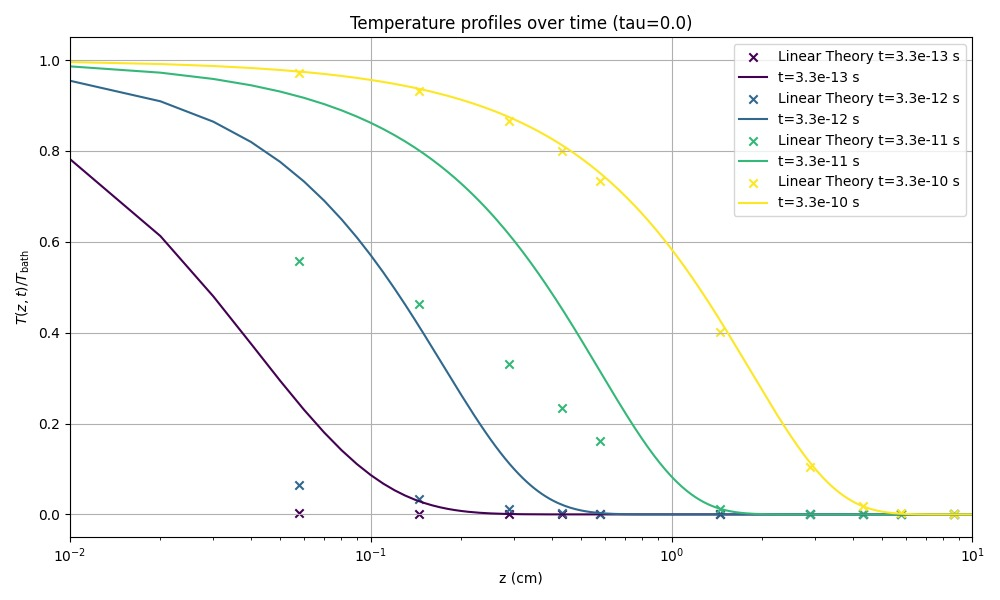
\includegraphics[width=0.8\textwidth]{Figures/Linear_case_comparison_Chi10000.png}
    \caption{comparison of the 1D diffusion linear code to the self-similar code where $\chi=10^4$ in the self-similar case.}
    \label{fig:Linear_case_comparison_chi10000}
\end{figure}
\begin{figure}[H]
    \centering
    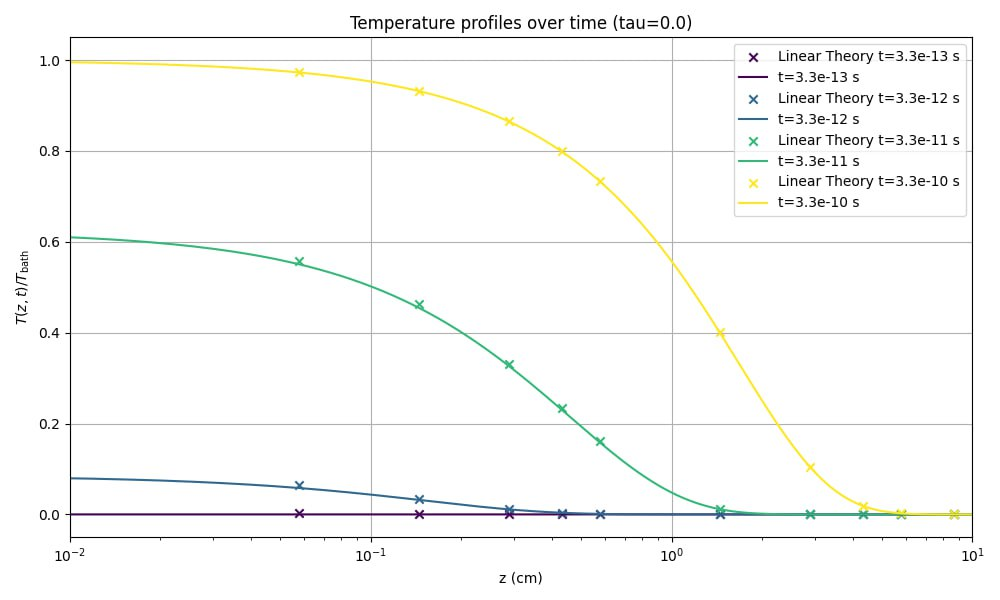
\includegraphics[width=0.8\textwidth]{Figures/Linear_case_comparison.png}
    \caption{comparison of the 1D diffusion linear code to the self-similar code where $\chi=1$ in the self-similar case.}
    \label{fig:linear_case_comparison_chi1}
\end{figure}


\subsection{Self-Similar Case in Gold}
<<<<<<< HEAD
The self-similar case in gold was tested against the semi-analytic solution provided in the Shussman and Heizler paper.
The comparisons were done for 2 different values of $\tau$: $\tau = 0$ and $\tau = 0.1408$. That because the Shussman and Heizler paper provided results for these 2 values of $\tau$, where $\tau=0$ is constant temperature boundary condition, and $\tau=0.1408$ is constant flux boundary condition.
The comparisons were done for the front position and for the total energy in the material, where they were calculated in the following way:
\begin{gather}
    z_f(t) = z \quad \mathrm{where} \quad \frac{\partial T(z_f,t)}{\partial z} \text{ is maximal} \\
    E_{total}(t) = \int_0^{z_F(t)} U_m(z,t) dz 
\end{gather}
The equations for the front position and total energy were taken from the Shussman and Heizler paper. For $tau = 0$:
\begin{gather}
    z_f(t) = 11.53\cdot 10^{-4} \rho_0^{-1.03}T^{1.95}t^{0.5} \\
    E_{total}(t) = 0.29 \rho_0^{-0.17}T^{3.55}t^{0.5}
\end{gather}
And for $\tau = 0.1408$:
\begin{gather}
    z_f(t) = 8.79\cdot 10^{-4} \rho_0^{-1.03}T^{1.95}t^{0.775} \\
    E_{total}(t) = 0.21 \rho_0^{-0.17}T^{3.55}t
\end{gather}
For $N_z = 1000$ and a changing time step ($dt_0=5\cdot 10^{-15}$ and $dt_{max} = 5\cdot 10^{-13}$), the results matched very well, as seen in figures \ref{fig:front_tau0_comparison}, \ref{fig:front_tau0.1408_comparison}, \ref{fig:energy_tau0_comparison} and \ref{fig:energy_tau0.1408_comparison}, for $Nz=10000$ the results were even better (not shown). 
=======
The self-similar case in gold was tested against the semi-analytic solution provided in the Shussman and Heizler paper. 
>>>>>>> d1caee19035fa5e340e10bfd1a28016377da5c2c
\begin{figure}[H]
    \centering
    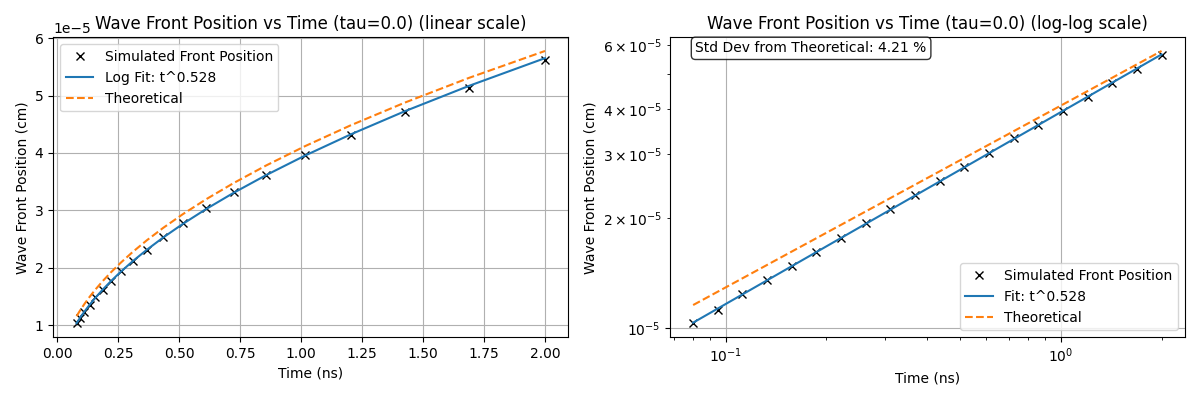
\includegraphics[width=0.8\textwidth]{Figures/front_tau0_comparison.png}
    \caption{comparison of the front position ($\tau = 0$) of the heat wave from 1D diffusion self-similar code to the Shussman and Heizler semi-analytic solution in gold.}
    \label{fig:front_tau0_comparison}
\end{figure}

\begin{figure}[H]
    \centering
    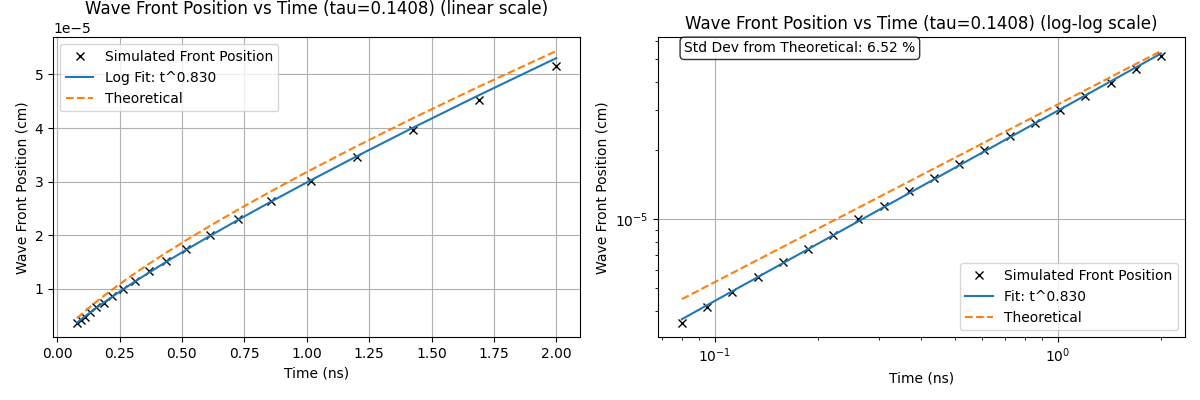
\includegraphics[width=0.8\textwidth]{Figures/front_tau0.1408_comparison.png}
    \caption{comparison of the front position ($\tau = 0.1408$) of the heat wave from 1D diffusion self-similar code to the Shussman and Heizler semi-analytic solution in gold.}
    \label{fig:front_tau0.1408_comparison}
\end{figure}

\begin{figure}[H]
    \centering
    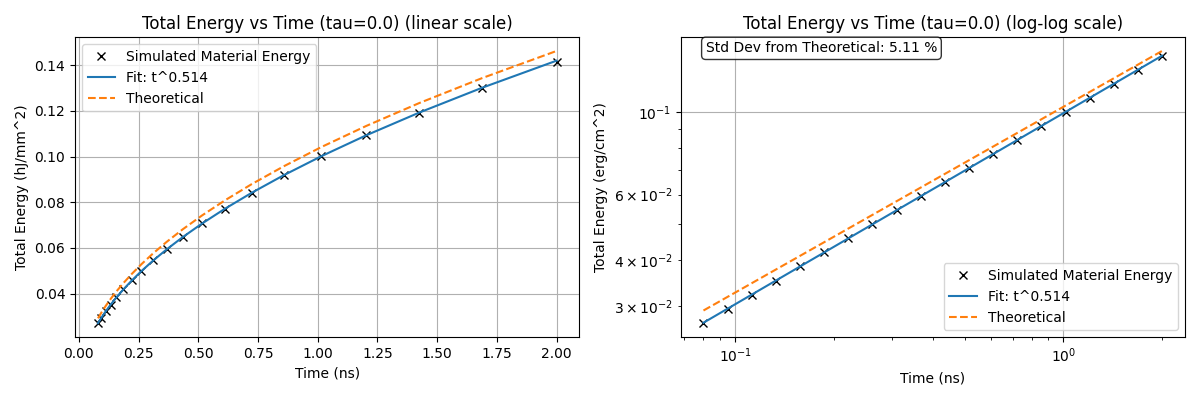
\includegraphics[width=0.8\textwidth]{Figures/energy_tau0_comparison.png}
    \caption{Comparison of the total energy ($\tau = 0$) from 1D diffusion self-similar code to the Shussman and Heizler semi-analytic solution in gold.}
    \label{fig:energy_tau0_comparison}
\end{figure}

\begin{figure}[H]
    \centering
    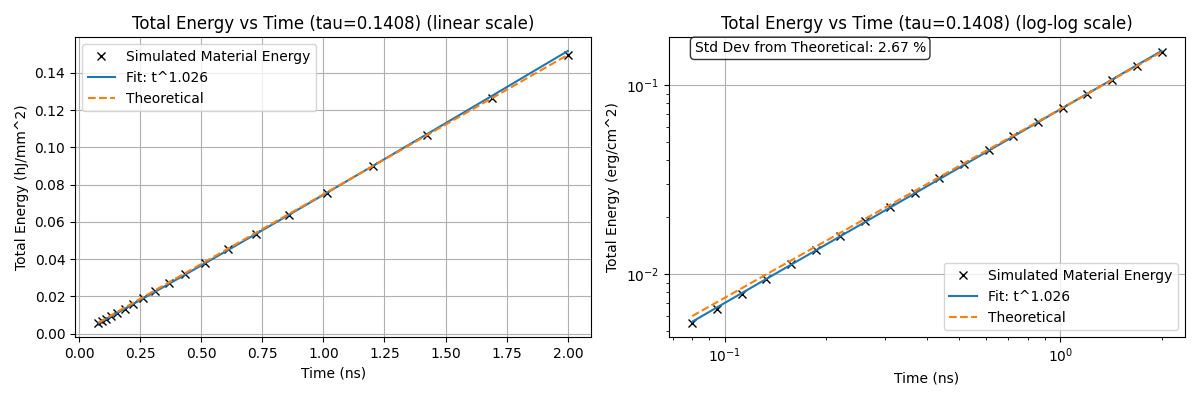
\includegraphics[width=0.8\textwidth]{Figures/energy_tau0.1408_comparison.png}
    \caption{Comparison of the total energy ($\tau = 0.1408$) from 1D diffusion self-similar code to the Shussman and Heizler semi-analytic solution in gold.}
    \label{fig:energy_tau0.1408_comparison}
\end{figure}


\end{document}
